\begin{frame}
    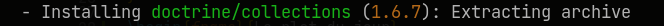
\includegraphics[width=\textwidth]{screenshots/Screenshot_20210520_104535.png}
\end{frame}

\begin{frame}
    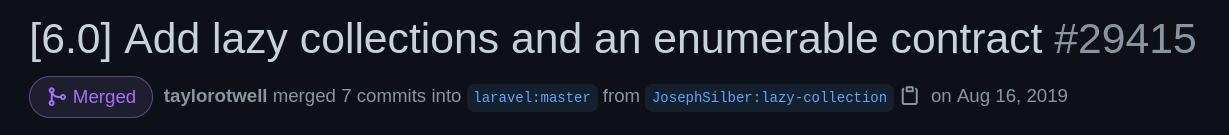
\includegraphics[width=\textwidth]{screenshots/Screenshot_20210520_101402.png}
    
\includegraphics[width=\textwidth]{screenshots/Screenshot_20210520_101458.png}
\end{frame}

\begin{frame}{Pourquoi}{Oui mais...}
    Tout cela est déjà possible avec des simples boucles.

    En effet.

    Il y a plusieurs types de profils.
    - Les business
    - Les passionnes

    L'avantage du business c'est qu'il delivre vite
    L'avantage des passionnes c'est qu'il favoriseront plutot
    des aspects comme la sémantique et la lisibilite du code.

    Les désavantages ne sont pas nécessaires ici, je laisse aux
    participants le soin de tirer leurs conclusions.

    Du coup, comme je me situe dans le dernier profil, j'ai cree
    loophp/collection.
\end{frame}

\begin{frame}{Pourquoi}{Motivations}
    \begin{itemize}[<+->]
        \item \colorbox{yellow}{\textbf{Personnelles}}, experimentation, \textit{learning-by-doing}
        \item Aider a mieux \colorbox{yellow}{\textbf{comprendre}} les concepts
        \item \colorbox{yellow}{\textbf{Simplifier}} l'utilisation de ces concepts
        \item \colorbox{yellow}{\textbf{Corriger}} un manquement (besoin $\Rightarrow$ solution)
        \item Et pourtant...
    \end{itemize}
\end{frame}

\begin{frameC}{Pourtant, on a déjà tout en PHP!}{Etat des lieux}

\end{frameC}

\begin{frame}{Pourquoi}{Gérer des ensembles de données}
    PHP dispose de \colorbox{yellow}{\textbf{fonctions natives}} propices à l'itération

    \pause

    \begin{itemize}[<+->]
        \item Les fonctions \texttt{array\_*} (\textit{$\pm$ 52 disponibles})
        \begin{itemize}[<+->]
            \item \texttt{array\_map()}
            \item \texttt{array\_filter()}
            \item \texttt{array\_reduce()}
            \item \texttt{array\_walk()}
        \end{itemize}
    \item \texttt{iterator\_to\_array()}
    \end{itemize}
\end{frame}

\begin{frame}{Pourquoi}{Gérer des ensembles de données}
    PHP dispose de \colorbox{yellow}{\textbf{structures natives}} propices à l'itération

    \pause

    \begin{itemize}[<+->]
        \item Tableaux (\texttt{array})
        \item Objects/Interfaces (\texttt{ArrayObject}, \texttt{ArrayAccess})
        \item Itérateurs
        \item Générateurs
    \end{itemize}
\end{frame}

\begin{frame}{Pourquoi}{Gérer des ensembles de données}
    PHP dispose de \colorbox{yellow}{\textbf{structures natives}} propices à l'itération

    \pause

    \begin{itemize}[<+->]
        \item \texttt{for}
        \item \texttt{foreach}
        \item \texttt{while}
        \item \texttt{do-while}
    \end{itemize}
\end{frame}

\begin{frameC}{Oui, mais\ldots}

\end{frameC}

\begin{frame}{Pourquoi}{Des incohérences dans les fonctions}
    \begin{itemize}
        \item \texttt{array\_map()}
        \item \texttt{array\_filter()}
        \item \texttt{array\_reduce()}
        \item \texttt{array\_walk()}
        \item \ldots
    \end{itemize}
\end{frame}

\begin{frame}{Pourquoi}{Des incohérences dans les fonctions}
    \begin{itemize}[<+->]
        \item Uniquement pour les \texttt{array}
        \item Inconsistance des fonctions (\texttt{array\_*()})
        \item Ordre des arguments (\textit{Sera probablement different avec PHP 8})
        \begin{itemize}[<+->]
            \item \texttt{array\_map(\$callable, \$array)}
            \item \texttt{array\_map(\$array, \$callable)}
        \end{itemize}
        \item Inconsistance des callbacks
        \item Pas de vérification des types
        \item Performances
        \item Pas de gestion des erreurs
    \end{itemize}
\end{frame}

\begin{frame}{Incohérences}{Exemple avec le célèbre \texttt{array\_map()}}
    En PHP, \texttt{array} est composé de \colorbox{yellow}{\textbf{couple(s)}} de\ldots

    \begin{itemize}[<+->]
        \item<1-> Clé
        \visible<3->{
            \begin{itemize}[<+->]
                \item Unique
                \item Type \texttt{integer} ou \texttt{string} uniquement
            \end{itemize}
        }
        \item<2-> Valeur
        \visible<4->{
            \begin{itemize}[<+->]
                \item Pas de restrictions ni sur l'unicité, ni sur les types
            \end{itemize}
        }

    \end{itemize}
\end{frame}

\begin{frameC}{Cependant\ldots}

\end{frameC}

\begin{frame}{Incohérences}{Exemple avec le célèbre \texttt{array\_map()}}
    \texttt{array\_map(callable \$callback, array \$array): array}

    \pause

    \begin{itemize}[<+->]
        \item \texttt{\$callback}

        \begin{itemize}[<+->]
            \item \texttt{callable} qui n'accepte qu'\colorbox{yellow}{\textbf{une seule}} valeur
        \end{itemize}

        \item \texttt{\$array}

        \begin{itemize}[<+->]
            \item N'accepte que les valeurs de type \colorbox{yellow}{\texttt{\textbf{array}}}
        \end{itemize}

        \item Retourne un \texttt{array}
    \end{itemize}

\end{frame}

\begin{frame}{Incohérences}{Exemple avec le célèbre \texttt{array\_map()}}
    \colorbox{yellow}{\textbf{Pourquoi}} alors la clé n'est elle pas passée à \texttt{\$callback} ?

    \begin{center}
        \includegraphics[width=.75\textwidth]{meme/b5p0aqqs1qc51.png}
    \end{center}
\end{frame}

\begin{frameC}{Bref\ldots}

\end{frameC}

\begin{frame}{Pourquoi}{Bref\ldots}
    \begin{itemize}[<+->]
        \item On \colorbox{yellow}{\textbf{sait}} que PHP n'est pas parfait\ldots \pause[\thebeamerpauses] mais qu'il va bientôt l'être!\pause
        \item On a \colorbox{yellow}{\textbf{l'habitude}}\ldots \pause[\thebeamerpauses] et donc, on ne fait plus attention
        \item Cela ne nous empêche pas de construire de \colorbox{yellow}{\textbf{belles choses}} malgré tout
    \end{itemize}
\end{frame}
